%%%%%%% Lecture Notes Style for Concrete Mathematics %%%%%%%%%%%%%
%%%%%%% Taught by Patrick White, TJHSST %%%%%%%%%%%%%%%%%%%%%%%%%%

% \documentclass[11pt,twosided]{article}
% %%%%%%%%%%%%%%%%%%%%%%%%%%%%%%%%%%%%%%%%%%%%%%%%%%%%%%%
%%%% HEADER FILE for CONCRETE MATH LECTURE NOTES %%%%%%
%%%%%%%%%%%%%%%%%%%%%%%%%%%%%%%%%%%%%%%%%%%%%%%%%%%%%%%

%%%%%%%%%%%%%%%%%%%%%%%%%%%%%%%%%%%%%%%%%%%%%%%%%%%%%%%%%%%%%%%%%%%
%% This file is included at the top of every lecture notes file %%%
%% It should ONLY be changed by the instructor %%
%%%%%%%%%%%%%%%%%%%%%%%%%%%%%%%%%%%%%%%%%%%%%%%%%%%%%%%%%%%%%%%%%%%

%%%%%%%%%%%%%%%%%%%%%% package inclusions %%%%%%%%%%%%%%%%%%%%
%\usepackage[
%top=2cm,
%bottom=2cm,
%left=3cm,
%right=2cm,
%headheight=17pt, % as per the warning by fancyhdr
%includehead,includefoot,
%heightrounded, % to avoid spurious underfull messages
%]{geometry} 


\usepackage{amsmath,amssymb,amsfonts}
\usepackage{longtable}
\usepackage{mathtools}
\usepackage{amsthm}
\usepackage{enumerate}
\usepackage{fancyhdr}
\pagestyle{fancy}


%%%%%%%%%%%%%%% theorem style definitions %%%%%%%%%%%%%%%%%%%%%%
\newtheorem{theorem}{Theorem}[section]
%\newtheorem{corollary}{Corollary}[theorem]
%\newtheorem{lemma}[theorem]{Lemma}
\newtheorem*{remark}{Remark}
%\newtheorem{example}{Example}[section]
\newtheorem*{definition}{Definition}


%%%%%%%%%%%%%%%% custom function definitions %%%%%%%%%%%%%%%%%%%%%%%%%
%%%%%%%%%%% as class progresses, this section may be enhanced %%%%%%%%

\def\multiset#1#2{\ensuremath{\left(\kern-.3em\left(\genfrac{}{}{0pt}{}{#1}{#2}\right)
		\kern-.3em\right)}} %%% multiset notation
\newcommand\rf[2]{{#1}^{\overline{#2}}} %%%% rising factorial \rf{x}{m}
\newcommand\ff[2]{{#1}^{\underline{#2}}} %%%%% falling factorial \ff{x}{m}
\newcommand{\Perm}[2]{{}^{#1}\!P_{#2}} % permutation
\newcommand{\half}{\ensuremath{\frac{1}{2}}}
\newcommand{\braces}[1]{\left\{#1\right\}}
\newcommand{\set}[1]{\braces{#1}}
\newcommand{\snb}[2]{\ensuremath{\left(\kern-.3em\left(\genfrac{}{}{0pt}{}{#1}{#2}\right)\kern-.3em\right)}}
\newcommand{\fallingfactorial}[1]{^{\underline{#1}}}
\newcommand{\fallfac}[2]{{#1}^{\underline{#2}}}
\newcommand{\stirlingone}[2]{\genfrac[]{0pt}{1}{#1}{#2}}
\newcommand{\stiri}[2]{\stirlingone{#1}{#2}}
\newcommand{\dstirlingone}[2]{\genfrac[]{0pt}{0}{#1}{#2}}
\newcommand{\dstiri}[2]{\dstirlingone{#1}{#2}}
\newcommand{\stirlingtwo}[2]{\genfrac\{\}{0pt}{1}{#1}{#2}}
\newcommand{\stirii}[2]{\stirlingtwo{#1}{#2}}
\newcommand{\dstirlingtwo}[2]{\genfrac\{\}{0pt}{0}{#1}{#2}}
\newcommand{\dstirii}[2]{\dstirlingtwo{#1}{#2}}
\newcommand{\ol}[1]{\overline{#1}}
%%%%%%%
% book stuff
%%%%%%%%%

\usepackage[twoside,outer=1.5in,inner=2in,bottom=1.5in,top=1.5in,marginpar=2in]{geometry} 
\usepackage{scrextend}
\usepackage{palatino}
\usepackage{multicol}
\usepackage{float}
\usepackage[hidelinks]{hyperref}
\usepackage[nameinlink, capitalise, noabbrev]{cleveref}
%\usepackage{background}
\usepackage{graphicx}
\usepackage{listliketab}

\usepackage{lipsum}
\usepackage{caption}
\usepackage{marginnote}

\reversemarginpar


\usepackage[dvipsnames]{xcolor}
\usepackage{amsthm}
\usepackage{shadethm}

\setlength{\parindent}{0pt}

\newcommand*\Note{%
	\marginnote[\textcolor{blue}{\raggedright{\LARGE ?}\ Note }]{}%
}
\newcommand*\Warn{%
	\marginnote[\textcolor{red}{\raggedright{\LARGE !}\ Warning }]{}%
}
\reversemarginpar

\newcommand{\N}{\mathbb{N}}
\newcommand{\Z}{\mathbb{Z}}
\newcommand{\I}{\mathbb{I}}
\newcommand{\R}{\mathbb{R}}
\newcommand{\Q}{\mathbb{Q}}
\renewcommand{\qed}{\hfill$\blacksquare$}
\let\newproof\proof
\renewenvironment{proof}{\begin{addmargin}[1em]{0em}\begin{newproof}}{\end{newproof}\end{addmargin}\qed}
% \newcommand{\expl}[1]{\text{\hfill[#1]}$}


\newenvironment{lemma}[2][Lemma]{\begin{trivlist}
		\item[\hskip \labelsep {\bfseries #1}\hskip \labelsep {\bfseries #2.}]}{\end{trivlist}}
\newenvironment{problem}[2][Problem]{\begin{trivlist}
		\item[\hskip \labelsep {\bfseries #1}\hskip \labelsep {\bfseries #2.}]}{\end{trivlist}}
\newenvironment{example}[2][Example]{\begin{trivlist}
		\item[\hskip \labelsep {\bfseries #1}\hskip \labelsep{\bfseries #2.}]}{\end{trivlist}}
\newenvironment{solution}{{\noindent \bfseries Solution\hskip 2ex}}{\qed}
\newenvironment{exercise}[2][Exercise]{\begin{trivlist}
		\item[\hskip \labelsep {\bfseries #1}\hskip \labelsep {\bfseries #2.}]}{\end{trivlist}}
\newenvironment{reflection}[2][Reflection]{\begin{trivlist}
		\item[\hskip \labelsep {\bfseries #1}\hskip \labelsep {\bfseries #2.}]}{\end{trivlist}}
\newenvironment{proposition}[2][Proposition]{\begin{trivlist}
		\item[\hskip \labelsep {\bfseries #1}\hskip \labelsep {\bfseries #2.}]}{\end{trivlist}}
\newenvironment{corollary}[2][Corollary]{\begin{trivlist}
		\item[\hskip \labelsep {\bfseries #1}\hskip \labelsep {\bfseries #2.}]}{\end{trivlist}}

% %%%% add package inclusions here, if any
% \usepackage{graphicx}
% \usepackage{xcolor}
% \usepackage{gensymb}
% %%%%% Define your custom functions and macros here, if any

% %%%%%%%%%%%%%%%%%%%% Define the variables below %%%%%%%%%%%%%%%%%%%%%%%%%%%%%%
% \def\titlestring{Catalan Numbers}
% \def\scribestring{Maguire Papay}
% \def\datestring{19, February, 2019}


%%%%%%%%%%%%%%%%%%% Page Headers -- Do Not Change %%%%%%%%%%%%%%%%%%%%%%%%%%%
% \lhead{\titlestring}
% \rhead{Page \thepage}
% \cfoot{Concrete Math -- White -- TJHSST}
% \renewcommand{\headrulewidth}{0.4pt}
% \renewcommand{\footrulewidth}{0.4pt}

% %%%%%%%%%%%%%%%%% Begin the document %%%%%%%%%%%%%%%%%%%%%%%%%
% \begin{document}
% \thispagestyle{plain}  %% no headers on this page

% %%%% Do not change these lines %%%%%
% \noindent
% {\LARGE \textbf{\titlestring}}\\\\
% %
% {\Large Scribe: \scribestring}\\ \\
% {\textbf{Date}: \datestring}


%%%%%%%%%%%%%%%%%%%%%%%%%% YOUR CONTENT GOES HERE %%%%%%%%%%%%%%%%%%%%%%%%%%
% \noindent

\section{Deriving the Numbers}
Q: How many triangulations are there of a labeled hexagon? (This means that although two triangulations may be the same under rotation, which vertices they are attached to matter).\\
Let us first examine the general case of an n-gon and look at the behavior of the first few \footnote{http://mathworld.wolfram.com/CatalanNumber.html}.\\
\begin{figure}[h]
%   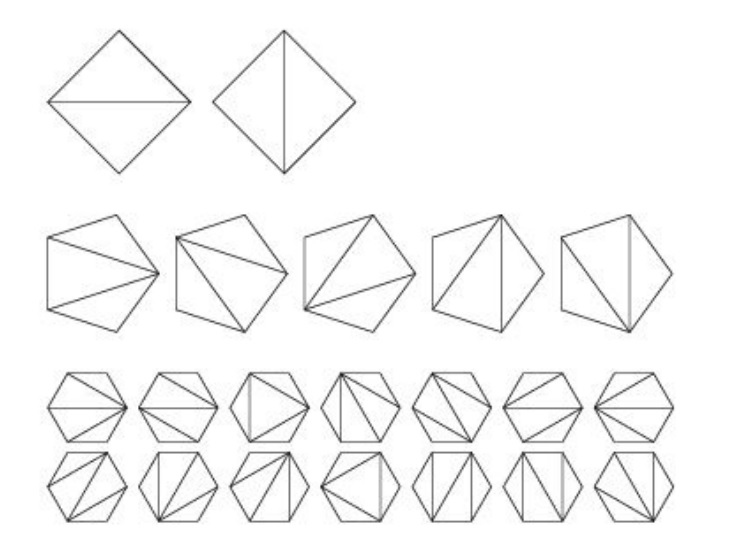
\includegraphics[width=\linewidth]{polygons.JPG}
  \caption{Triangulations for 4, 5, and 6 sided polygons.}
  \label{fig:triangs1}
\end{figure}\\
The rules for triangulation are only such that there are no crossings between the lines. Note: a triangulation of an n-gon uses n-3 line segments and results in n-2 interior triangles.\\
As we can see from Figure 1, the answer to our original question is 14, but let us instead try to come up with a general formula for $T_n = $ number of ways to $\triangle$ a n-gon.\\
\\
Note: The following graphics will be done in Microsoft Paint. I'm sorry in advance.\\


\begin{theorem}
	$$T_n = \sum_{k=2}^{n-1}T_{n-(k-1)}\cdot T_{k-1}$$
\end{theorem}
\begin{proof}
	\textcolor{red}{WARNING: THIS WAS THE PROOF THAT WAS SHOW IN CLASS THAT HAD AN ERROR IN IT. I still think it is worth to look it over and see why it doesn't work. Just to clarify, although this proof does give the correct recursion, it is not correct. To my knowledge, it is nothing short of a miracle that this method accidentally over-counts and under-counts solutions in such a way to produce a correct recursion.}
	\begin{figure}[h]
        % 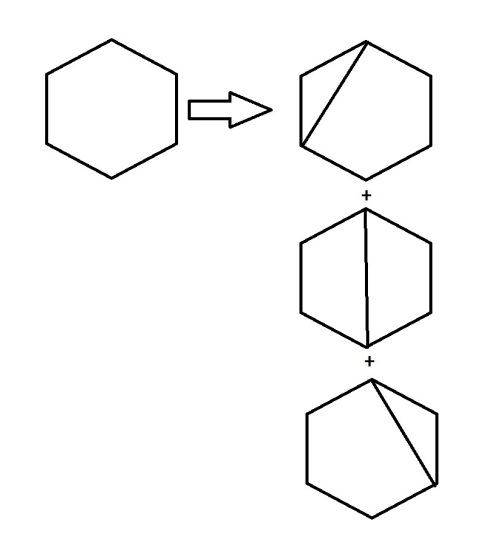
\includegraphics[width=\linewidth]{T6Hexagons.jpg}
        \caption{Recursion for a hexagon.}
        \label{fig:hex1}
    \end{figure}\\
    This hexagon could be broken up into 3 different shapes like this, which would result in $T_6 = T_3\cdot T_5 + T_4\cdot T_4 + T_5\cdot T_3$. This obviously satisfies our original theorem, and all n-gons could be split like this, but this does over-count, because it does not account for when splitting up the remaining polygons you end up with the same triangulation. That is the reason why this proof does not work well for formulating the Catalan numbers.
\end{proof}
\begin{proof}
    Instead of splitting the polygon with a line, which allows for over-counting, if it is instead split with a triangle, we are guaranteed that each solution found is unique, and from looking at the diagram below, we see that the sum of each of these will give us the correct number.
    \begin{figure}[h]
        % 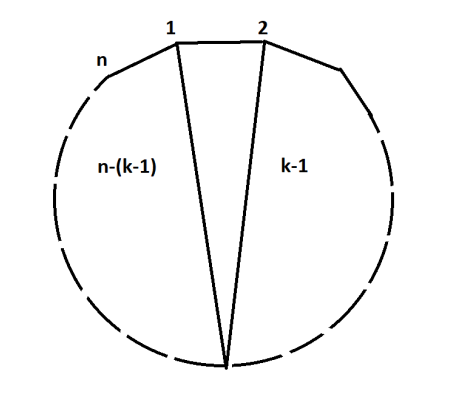
\includegraphics[width=\linewidth]{correctHexagon.png}
        \caption{Correct recursion for a hexagon.}
        \label{fig:hex2}
    \end{figure}\\
\end{proof}

\section{Deriving the Numbers: Part 2}
Q: How many paths are there between the points (0, 0) and (2n, 0), only moving with steps of either northeast (up one right one) or southeast (down one right one).\\ (Note: This is analogous to the question of paths between (0, 0) and (n, n) with only vertical and horizontal steps except the algebra works better in this one. However, the pictures I can find are using this interpretation of the problem, so unless we want more Microsoft Paint pictures, these will do. If at any point you get confused between what we did in class and the pictures I'm showing, turn your head $45^\circ$ to the left and it will make sense again.)\\
A: $\binom{2n} n$. 
\begin{proof}
    There are 2n moves, n of them must be up, n must be down, so choose which n will go southeast and we are done.\\
\end{proof}

\begin{figure}[h]
    % 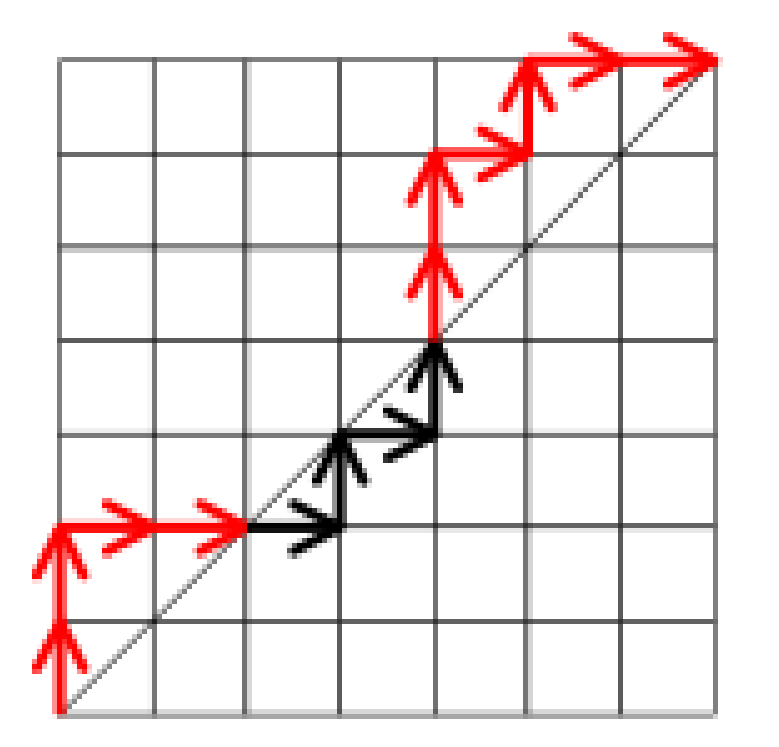
\includegraphics[width=\linewidth]{Catalan_number_exceedance_example.png}
    \caption{An example of a path.}
     \label{fig:hex3}
\end{figure}

Now we want to count all of the paths that do not cross the x-axis, as the one in Figure 4 does. I'm going to have to use paint for this as I cannot find pictures. Sorry again. 

In order to do this, we first notice that all bad paths (ones that cross the x axis), touch the line y = -1 at least once. To count them, we will reflect everything BEFORE the first y = -1 touch along the line y = -1, and leave everything after it the same. (This is why we do it this way instead of diagonally because the reflection is much easier to visualize). This creates a mapping of all bad paths to something else. This is a one to one mapping, every bad path has a reflection, and every reflection has only 1 bad path associated with it. Now, by counting the reflections we also count bad paths. Since the bad paths start at y = -2, and need to reach (2n, 0), we have to choose n+1 up moves (note that this is because this will also result in one less down move, leaving us two above our initial position). \\So bad paths = $\binom{2n}{n-1}$
\\
\\
This gives our total amount of good paths to be the following $$P = \binom{2n}{n} - \binom{2n}{n+1}$$ $$\frac{(2n)!}{n!\cdot n!}-\frac{(2n)!}{(n-1)!(n+1)!} = \frac{(2n)!}{n!\cdot n!} \cdot(1-\frac{n}{n+1})$$
$$= \frac{1}{n+1}\binom{2n} n$$
Which is the Catalan numbers (note how by splitting up the original path problem into two smaller ones, we can also achieve the recursion relation for the Catalan numbers, like we did with the hexagons).

\begin{figure}[h]
    % 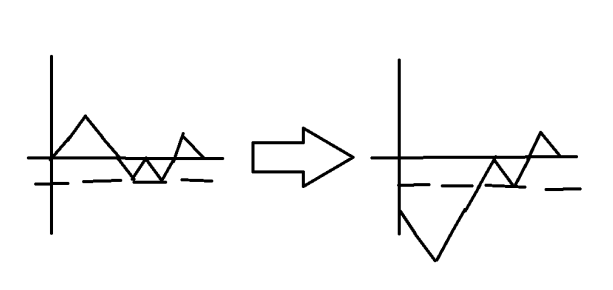
\includegraphics[width=\linewidth]{CatalanAgain.png}
    \caption{The transformation applied to all bad paths}
     \label{fig:hex4}
\end{figure}
% \end{document}
